% A quotient and its rounding cell. All distinctions survive grayscale printing.
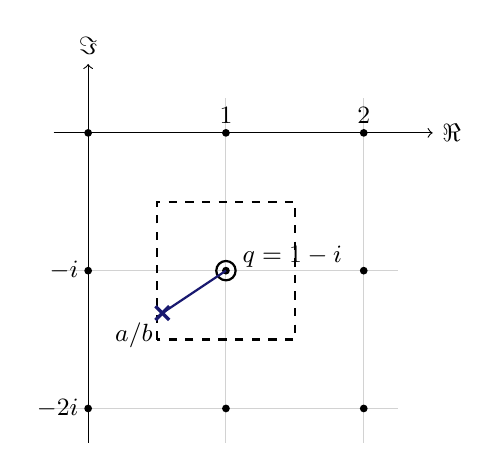
\begin{tikzpicture}[x=1.75cm,y=1.75cm,font=\small]
  \draw[step=1,gray!35] (-.25,-2.25) grid (2.25,.25);
  \draw[->] (-.25,0)--(2.5,0) node[right] {$\Re$};
  \draw[->] (0,-2.25)--(0,.5) node[above] {$\Im$};
  \foreach \x in {0,1,2} \foreach \y in {-2,-1,0} \fill (\x,\y) circle (1.4pt);
  \foreach \x in {1,2} \node[above] at (\x,0) {$\x$};
  \node[left] at (0,-1) {$-i$};
  \node[left] at (0,-2) {$-2i$};
  \draw[dashed,thick] (.5,-1.5) rectangle (1.5,-.5);
  \draw[thick] (1,-1) circle (3.5pt);
  \node[right] at (1.05,-.9) {$q=1-i$};
  \draw[very thick,MidnightBlue] ({7/13-.05},{-17/13-.05})--({7/13+.05},{-17/13+.05});
  \draw[very thick,MidnightBlue] ({7/13-.05},{-17/13+.05})--({7/13+.05},{-17/13-.05});
  \draw[thick,MidnightBlue] (7/13,-17/13)--(1,-1);
  \node[below left] at (7/13,-17/13) {$a/b$};
\end{tikzpicture}
